\documentclass[UTF8]{ctexart}
\usepackage{geometry}
\usepackage{indentfirst}
\usepackage{hyperref}
\usepackage{harpoon}
\usepackage{amsmath}
\usepackage{graphicx}
\usepackage{float}
\usepackage{subfigure}
\usepackage{multirow}
\usepackage{array}
\usepackage{tikz}
\usetikzlibrary{arrows, shapes, positioning, calc}
\geometry{a4paper, left=1cm, right=1cm, top=2cm, bottom=2cm}
\setlength{\parindent}{1cm}
\renewcommand\contentsname{Content}
\title{伊辛模型的蒙特卡洛数值计算}
\author{段元兴}
\date{\today}
\begin{document}
\maketitle
\thispagestyle{empty}
\setcounter{page}{1}
\newpage
\tableofcontents
\newpage
    \section{背景介绍}
        \indent 伊辛模型 (Ising model)是一个以物理学家恩斯特·伊辛为名的数学模型, 用于描述物质的铁磁性.
        该模型中包含了可以用来描述单个原子磁矩的参数 $\sigma _{i}$, 其值只能为+1或-1, 分别代表自旋向上或向下,
        这些磁矩通常会按照某种规则排列, 形成晶格, 并且在模型中会引入特定交互作用的参数, 使得相邻的自旋互相影响.
        虽然该模型相对于物理现实是一个相当简化的模型, 但它却和铁磁性物质一样会产生相变.
        事实上, 一个二维的方晶格伊辛模型是已知最简单而会产生相变的物理系统.\\
        \indent 伊辛模型最早是由物理学家威廉·楞次在1920年发明的, 他把该模型当成是一个给他学生恩斯特·伊辛的问题.
        伊辛在他一篇1924年的论文中求得了一维伊辛模型的解析解, 并且证明它不会产生相变. 二维方晶格伊辛模型相对于一维的难出许多,
        因此其解析的描述在一段时间之后才在1943年由拉斯·昂萨格给出. 一般来说, 二维伊辛模型的解析解可由传递矩阵法求得,
        不过也有几个和量子场论有关的解法. 对于大于三维的伊辛模型目前还没有找到解析解, 但其近似解可由诸多方法求得, 例如平均场论.\\
        \indent 这里, 我们不再讨论严格或平均场近似的理论计算方法, 而是利用计算机数值计算给出二维周期边界条件有外场的解,
        并观察其在不同温度和磁场下的各物理量的变化情况.
    \section{理论推导}
        \subsection{微正则系综}
            \indent 在开始准备写代码之前需要进行理论推导, 对推导结果采取不同的方式进行模拟并比较结果的差异. 对于一个伊辛模型系统,
            其哈密顿量可以写作:
            \begin{equation}
                H(\sigma)=-\sum\limits_{i,j}J_{ij}\sigma_i\sigma_j-\mu\sum\limits_jH_j\sigma_j
            \end{equation}
            其中$\sigma$代表的是整个自旋系统 (自旋组态), $J_{ij}$是不同晶格点相互作用的系数, 对于铁磁性物质$J_{ij}>0$, 对于反铁磁性物质$J_{ij}<0$,
            $H_j$是外加磁场. 这里模拟的二维伊辛模型的每个小磁矩仅与其周围上下左右4个磁矩有相互作用.\\
            \indent 该系统的的组态几率是
            \begin{equation}
                P(\sigma)=\dfrac{e^{-\beta H(\sigma)}}{\sum\limits_\sigma e^{-\beta H(\sigma)}}
            \end{equation}
            物理量$f(\sigma)$是自旋组态$\sigma$的函数, 其期望值 (系综平均)为
            \begin{equation}
                \langle f\rangle=\sum\limits_\sigma P(\sigma)f(\sigma)
            \end{equation}
        \subsection{蒙特卡洛 (Monte Carlo)算法}
            \indent 一个很简单的想法就是随机生成大量自旋系统来产生一个系综, 再按照上式来计算物理量的平均值.\\
            \indent 但是这种    想法显然弊端很大, 例如在温度$T\rightarrow 0$的时候铁磁性物质的自旋应该都是同向的, 但是对于一个$N$格点的系统,
            直接随机抽样得到自旋都同向的概率是$\dfrac{1}{2^{N-1}}$, 如果格点数量庞大, 例如256$\times$256的正方形网格, 直接抽样得到这样的系统几乎是不可能的,
            也即是说我们不可能得到正确的结果. 所以需要引入新的方法来进行数值计算.
        \subsection{梅特波利斯 (Metropolis)算法}
            \indent 既然直接等概率的采样所有系统行不通, 那么可不可以按照一定概率来采样? 例如既然自旋都相同的概率为1, 如果我们事先知道了这个系统的概率是1,
            采样时就可以直接选取这个系统然后计算:
            \begin{equation}
                \langle f\rangle=\dfrac{\sum\limits_\sigma^M f(\sigma)PP^{-1}}{\sum\limits_\sigma^M PP^{-1}}=\dfrac{\sum\limits_\sigma^M f(\sigma)}{M}
            \end{equation}
            其中$M$是总的采样数. 这被称之为重要性采样. 这个方法可以让最大概率的那些系统被采样的概率大大提升, 加速了整个系综平均收敛的速度.\\
            \indent 我们面临这样一个问题: 如何在不知道整个系统的情况下得到其产生的概率? 此时需要使用马尔可夫 (Markov)过程: 首先得到一个任意态,
            可以是随机产生的或者是同向的等等, 再设计这样一种过程: 从低概率态到达高概率态的概率大于从高概率态反过来到达低概率态的概率. 这样就能保证
            随着系统状态的不断迁移, 整个系统是朝着高概率态移动的, 在达到稳定的时候就能开始采样并计算各个物理量的系综平均. 但是这种系统迁移需要满足两个条件:\\
            \indent 1. 遍历性. 这个是为了满足整个整个系综都有可能被抽样的条件 (虽然有些低概率态永远不可能被抽样到).\\
            \indent 2. 细致平衡条件. 具体来说就是稳态时从一个态$A$迁移到其他能迁移到的态$B_i$的总概率
            \begin{equation}
                P(A)\sum\limits_iP(A\rightarrow B_i)
            \end{equation}
            等于从$B_i$迁移到$A$的总概率
            \begin{equation}
                \sum\limits_iP(B_i)P(B_i\rightarrow A),
            \end{equation}
            这样就满足了整个迁移过程的稳定性, 从某种角度可以理解为概率流的散度为0. 这里采取一种最简单的方式来满足细致平衡条件:
            \begin{equation}
                P(A)P(A\rightarrow B_i)=P(B_i)P(B_i\rightarrow A)
            \end{equation}
            直接将其带入即可验证这种迁移满足细致平衡条件. 对于这里的系统迁移, 可以直接算出
            \begin{equation}
                \dfrac{P(A\rightarrow B)}{P(B\rightarrow A)}=\dfrac{P(B)}{P(A)}=e^{\beta(E_A-E_B)}.
            \end{equation}
            \indent 最后, 根据细致平衡条件带来的对迁移概率限制可以设计出如下迁移概率:
            \begin{equation}
                P(A\rightarrow B)=
                \left\{
                    \begin{array}{ll}
                        e^{-\beta(E_B-E_A)}, &E_B-E_A>0\\
                        1, &E_B-E_A<=0\\
                    \end{array}
                \right.
            \end{equation}
    \section{计算方法}
        \subsection{随机采样}
            \indent 1. 生成一个随机态;\\
            \indent 2. 计算总能量$E$, 组态几率$P$, 物理量$f$等等;\\
            \indent 3. 随机翻转一个格点, 计算能量差从而得到新的能量$E'$, 重复2直到采样到足够多的系统;\\
            \indent 4. 计算物理量$f$的统计平均值.
        \subsection{马尔科夫链}
            \indent 1. 首先初始化一个态, 可以是随机的或者同向的等等;\\
            \indent 2. 随机选取一个格点, 计算翻转前后其与周围格点, 磁场相互作用能的改变, 按照上面推导得到的概率来判断是否翻转;\\
            \indent 3. 检查是否达到了高概率态并且系统总能量处于稳定状态, 如果是则可以开始采样系统了;\\
            \indent 4. 对采样得到的系统进行平均.
    \section{计算结果}
        \indent 这里将对不同尺寸 (边长$2^k$, $k=7,8,9,10$) 的周期边界正方形网格进行计算, 统计出各个物理量随着温度$T$, 磁场强度$H$的变化情况 (为了避免网格大小造成的绝对值变化,
        以下的各个物理量都已经除以了格点数量), 观察其热容, 磁化率和熵, 以及网格尺寸, 温度和平均时间对于零外场临界相变磁畴凝聚的影响和模拟磁滞曲线.
        \subsection{磁矩和能量}
            \subsubsection{磁矩$M$}
                \indent 这是边长256网格的$M(H,T)$图像:
                \begin{center}
                    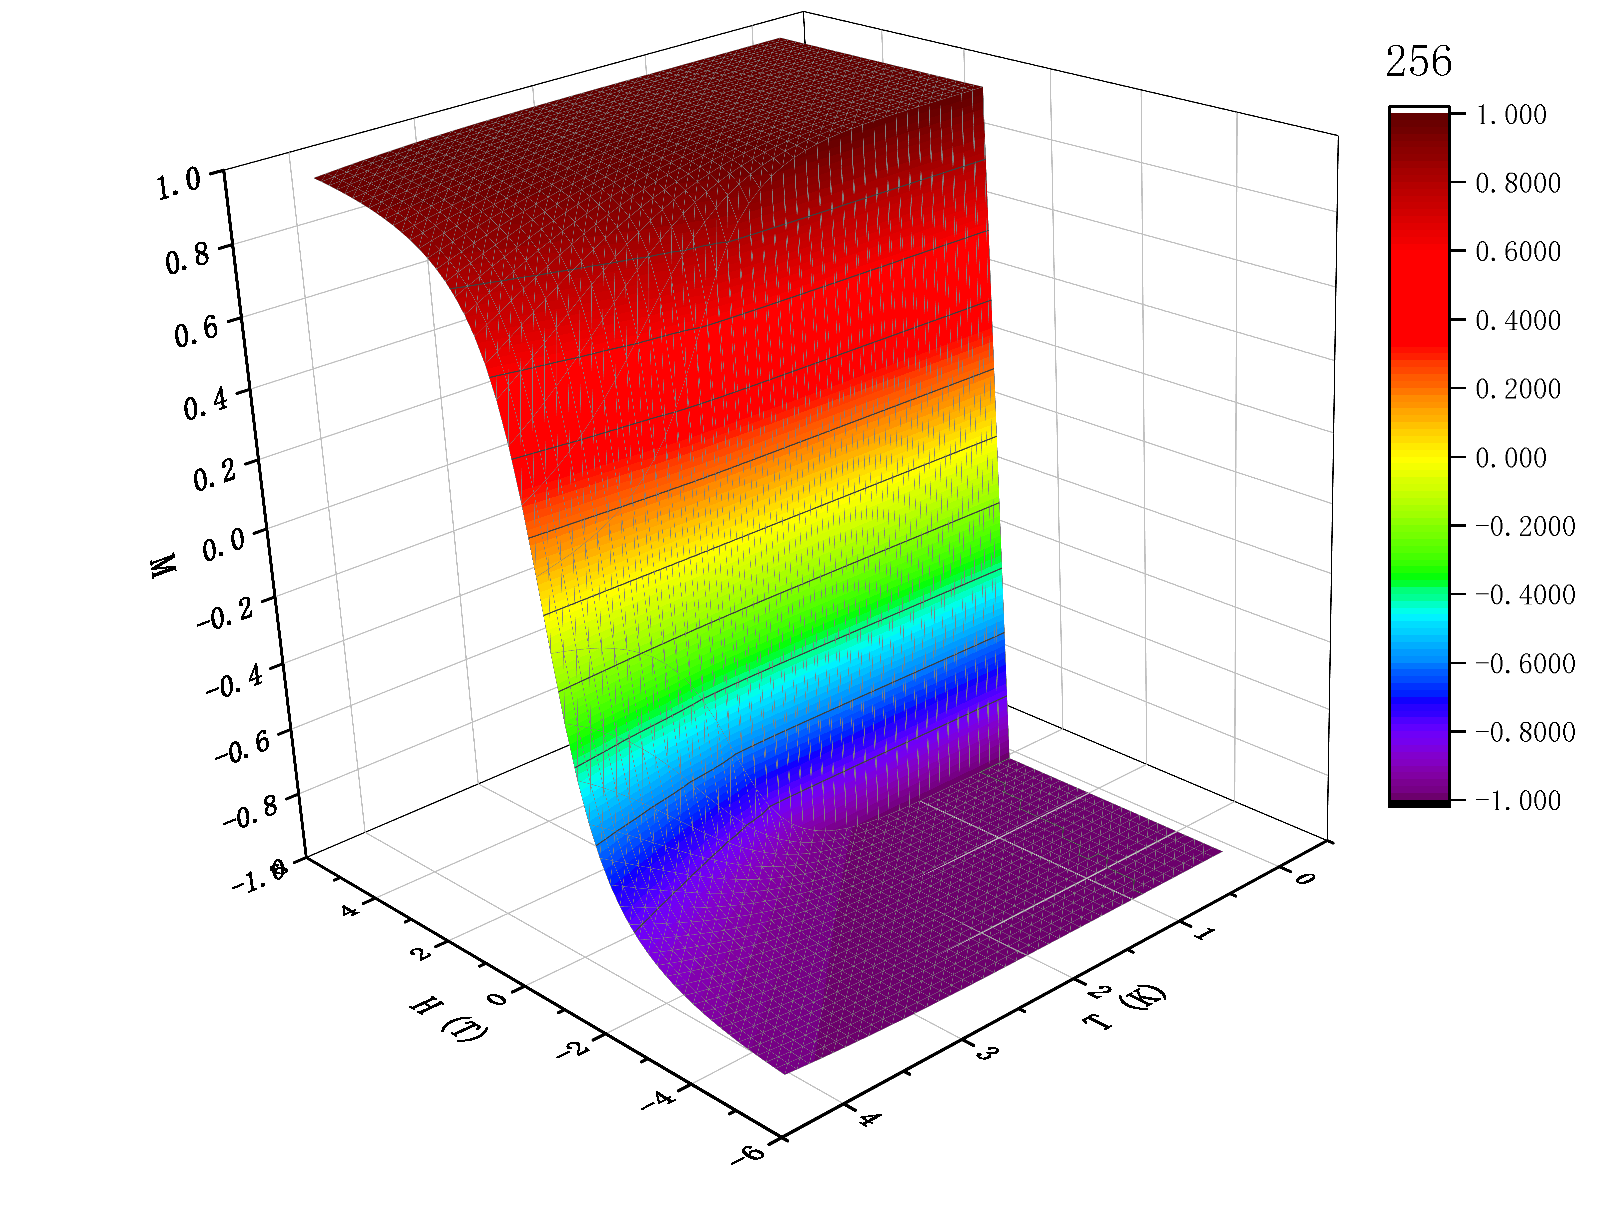
\includegraphics[width=17cm]{M-HT256.pdf}
                \end{center}
                可以在温度低于临界温度$T_c=2.268K$时发现明显的$M$不连续现象, 即意味着降温系统发生相变时磁矩的最终朝向是取决于外场方向的.\\
                \indent 而为了研究无外场下$T_c$附近磁矩与温度的关系, 经过提高分辨率和更多系统的平均, 并使用多次计算结果的平均, 得到以下结果:
                \begin{center}
                    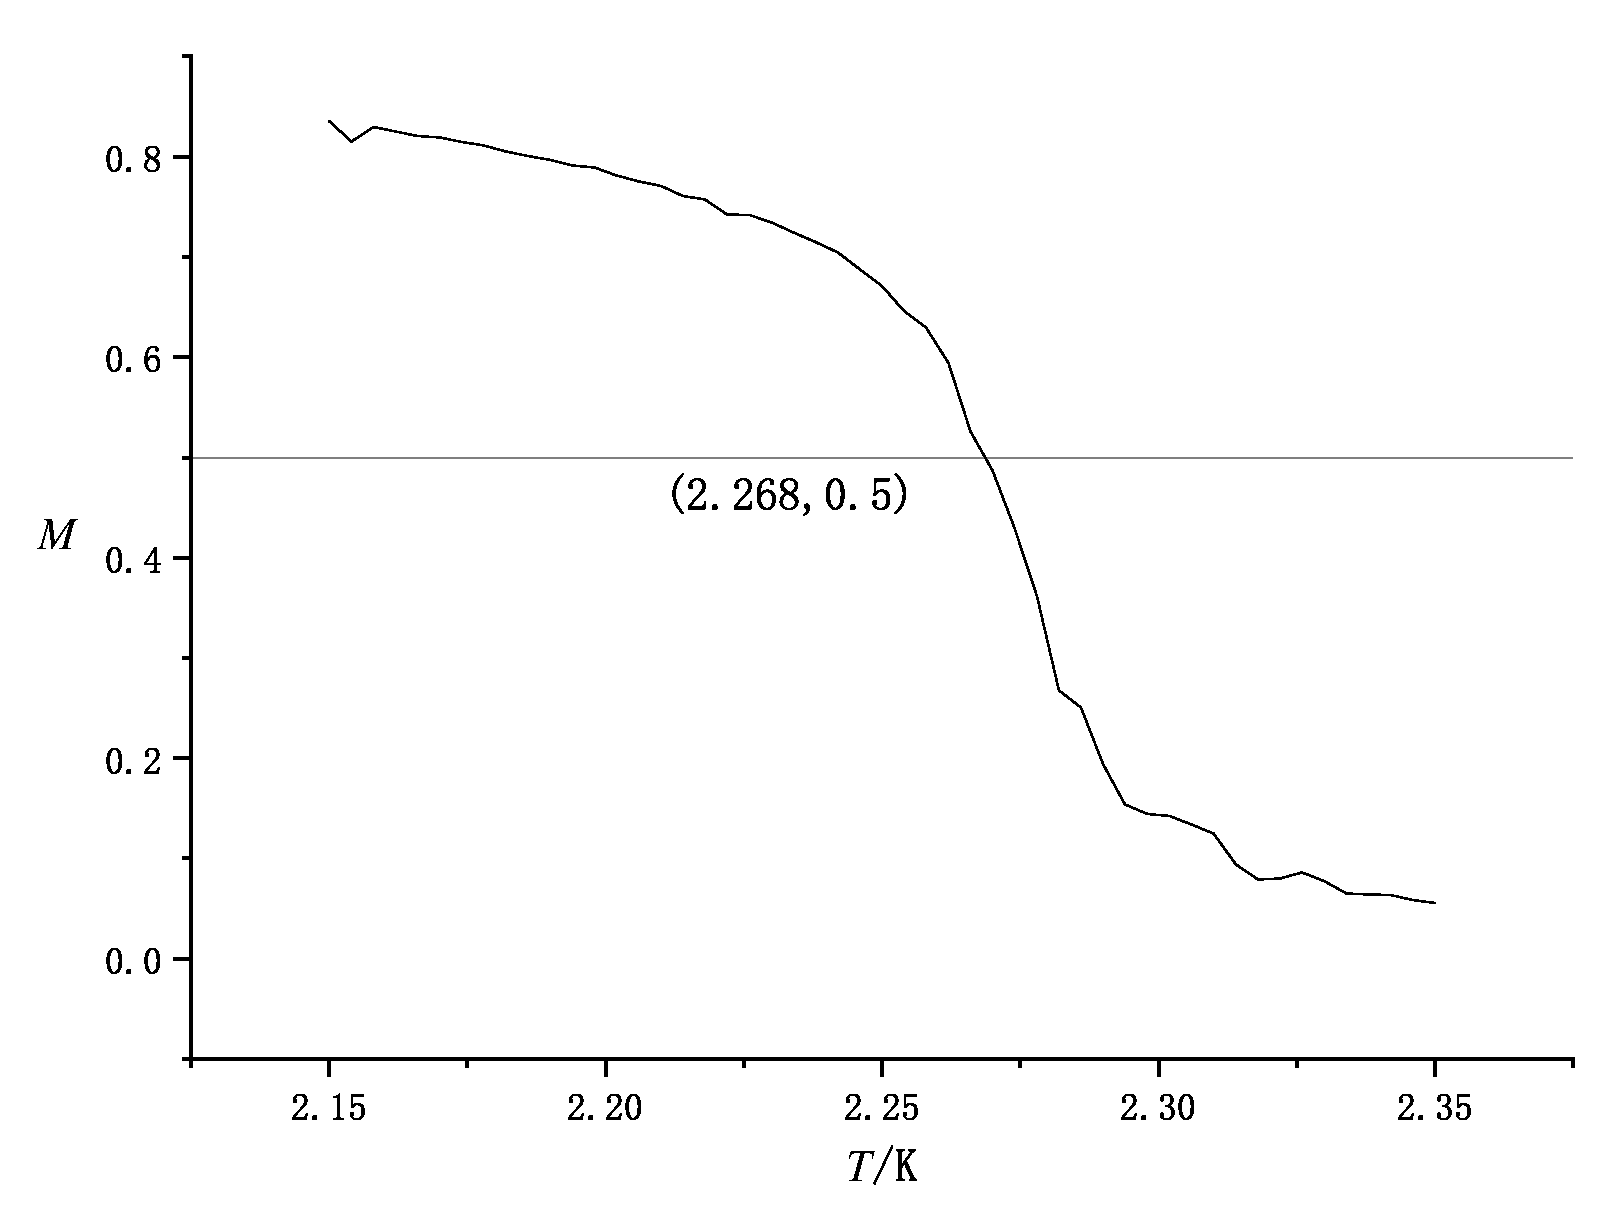
\includegraphics[width=10cm]{PhaseTransition.pdf}
                \end{center}
                \newpage
            \subsubsection{能量$E$}
                \indent 这是边长256网格的$E(H,T)$图像:
                \begin{center}
                    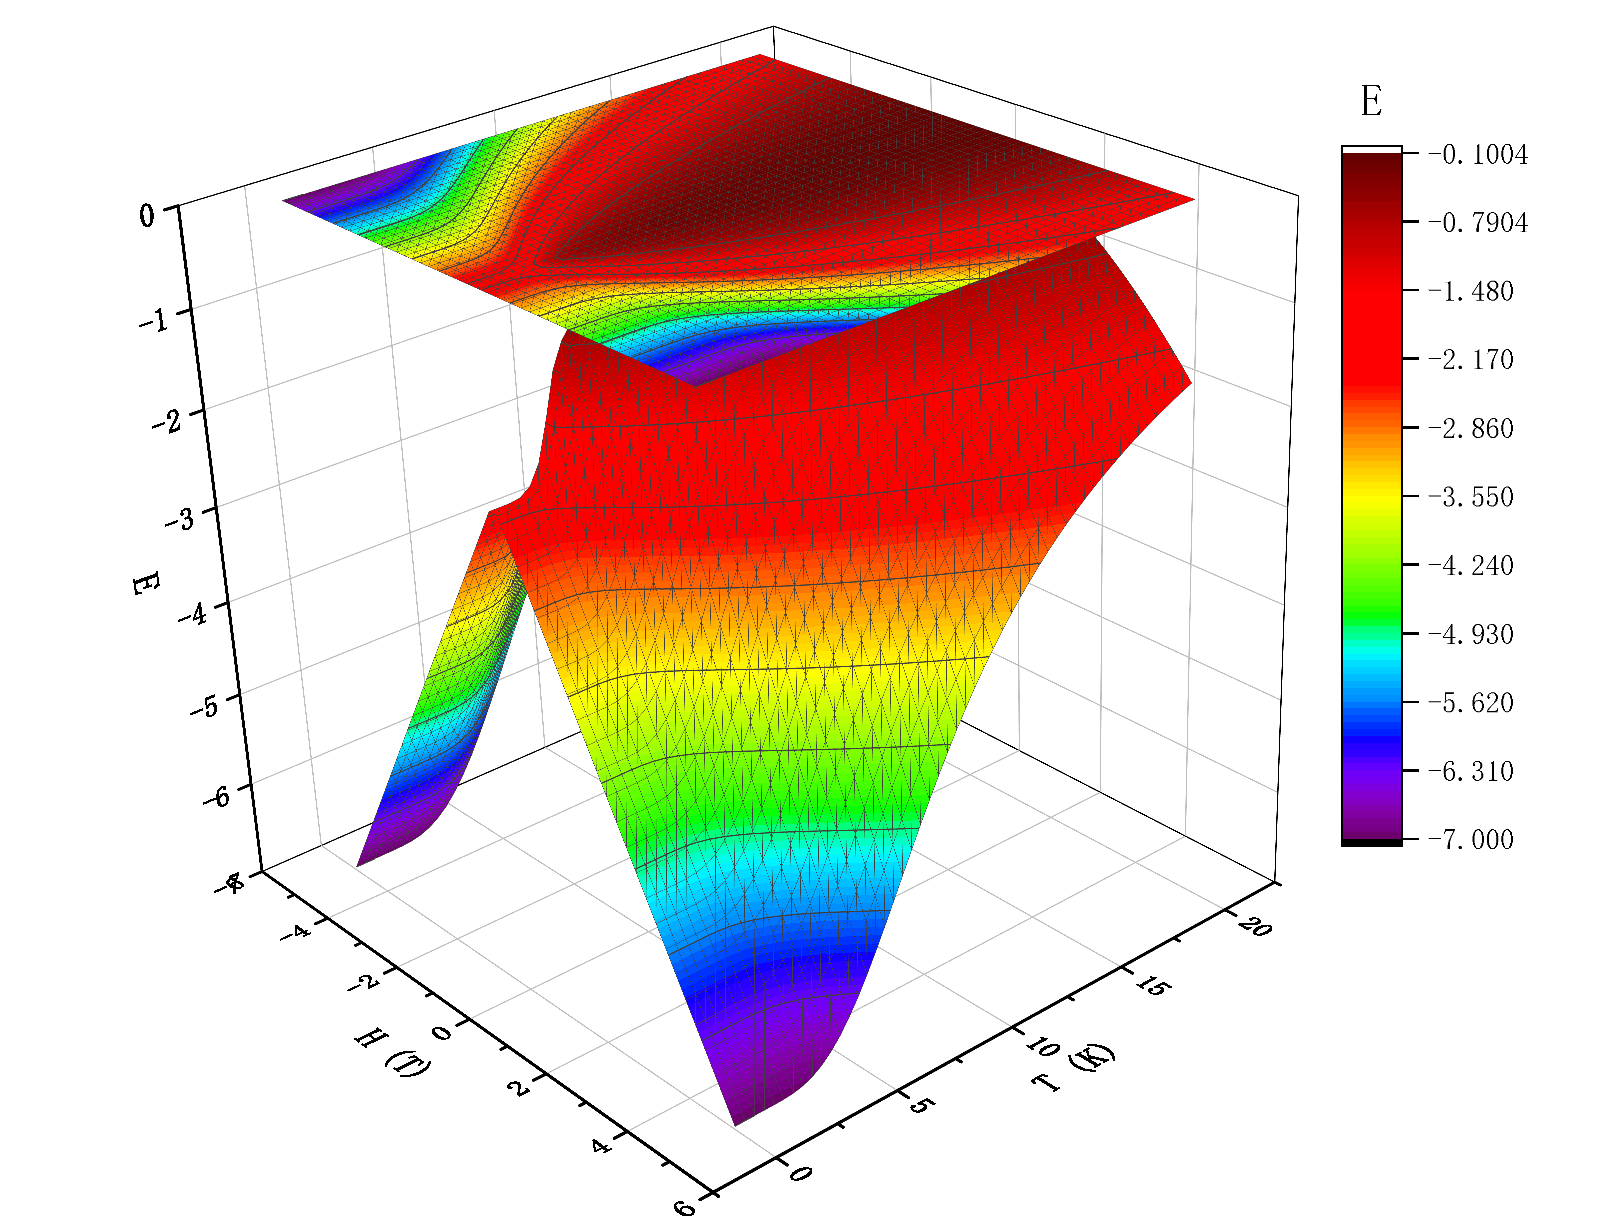
\includegraphics[width=17cm]{E-HT256.pdf}
                \end{center}
                这里发现系统能量随着温度的增加, 在$T_c$以下系统能量基本不变, 而在$T>T_c$时整个系统的能量开始迅速增加, 且这个增加的速率会随着磁场的增强减小, 物理上理解就是
                外场强行把整个系统的磁矩作用成与磁场同向的, 系统处于低能态, 所以需要更高的温度以增大磁矩翻转的概率, 使系统的能量增加. 从等能曲线上也能看出, 相同的能量下,
                磁场强度越强, 温度越高, 而且一系列等能曲线中间出现了一个分叉点, 那个点的温度就是$T_c$, 物理含义: 从该点开始系统能量若要继续降低, 则磁场 (即系统磁矩) 的方向必须是
                一个确定的方向, 即发生了相变.
                \newpage
            \subsubsection{网格尺寸的影响}
                \indent 为了观察尺寸对于模拟的影响, 这里作出相对于边长128网格各个尺寸网格的$M, E$绝对差值:
                \begin{figure}[H]
                    \centering
                    \subfigure{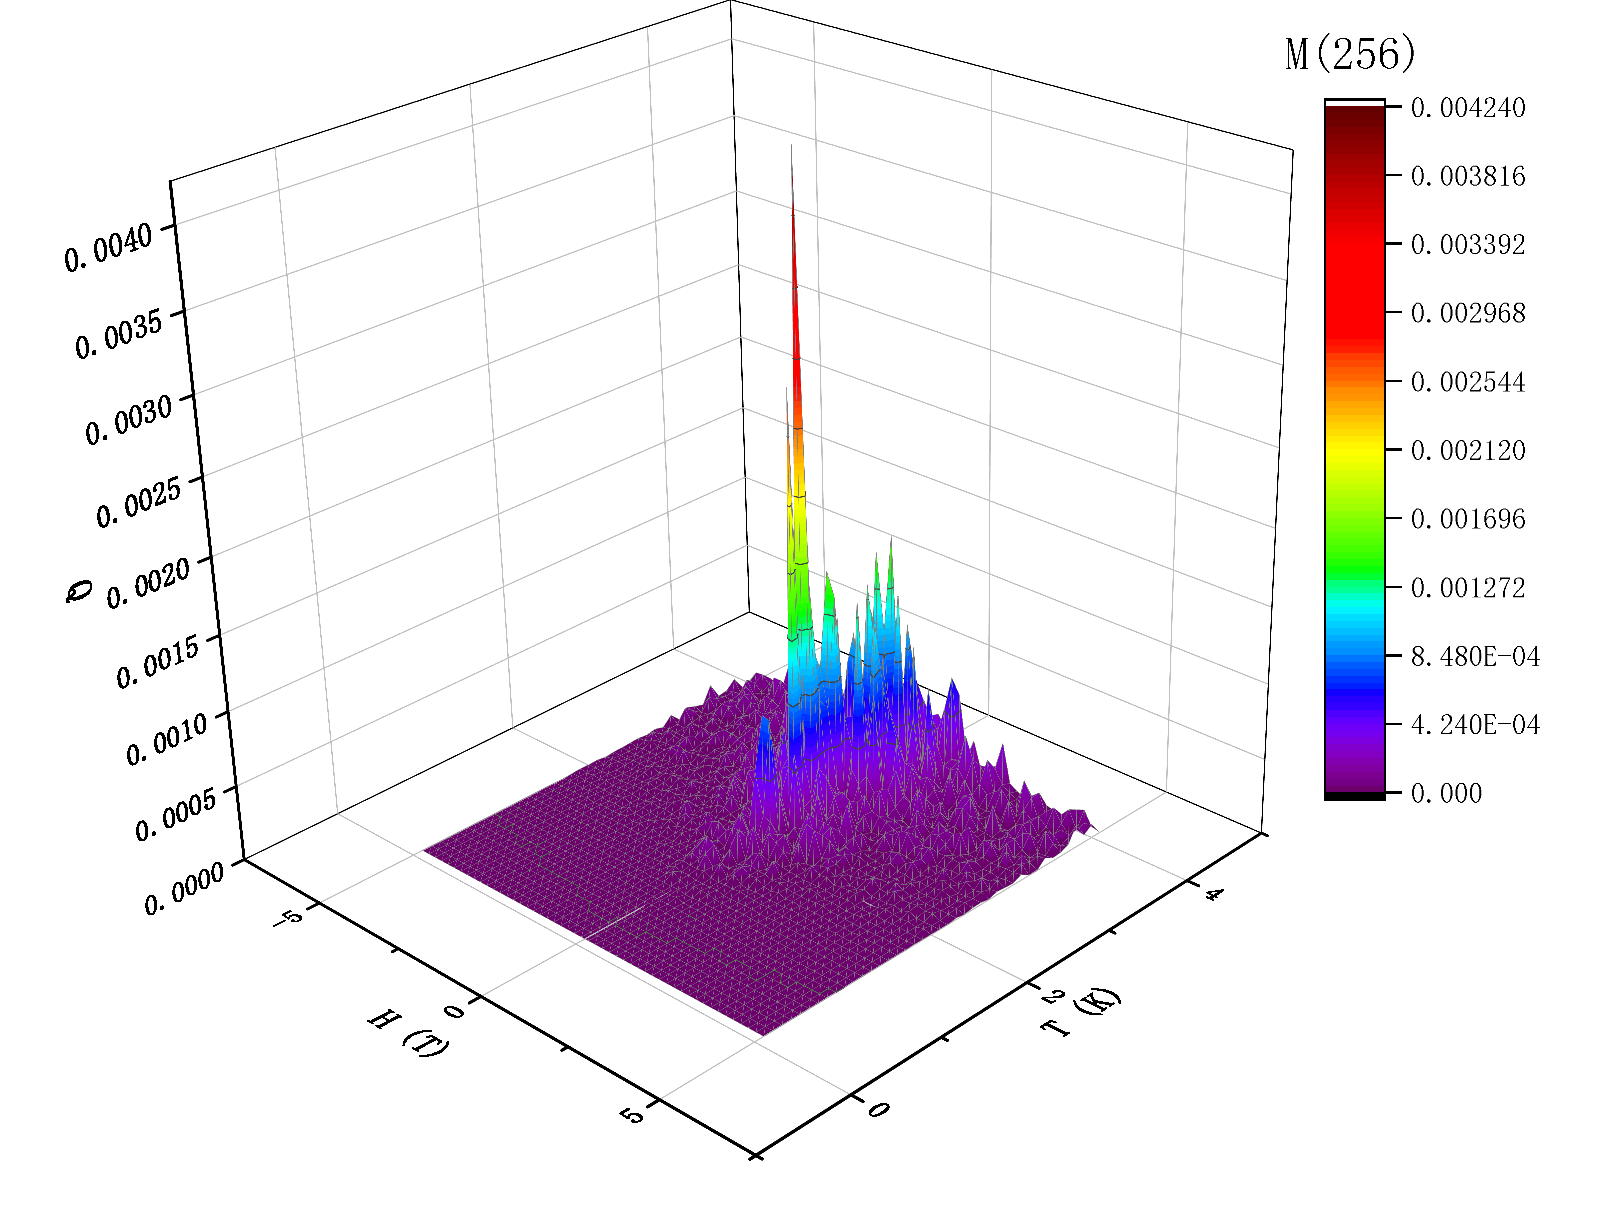
\includegraphics[width=5.5cm]{DeltaM-HT256.pdf}}\quad
                    \subfigure{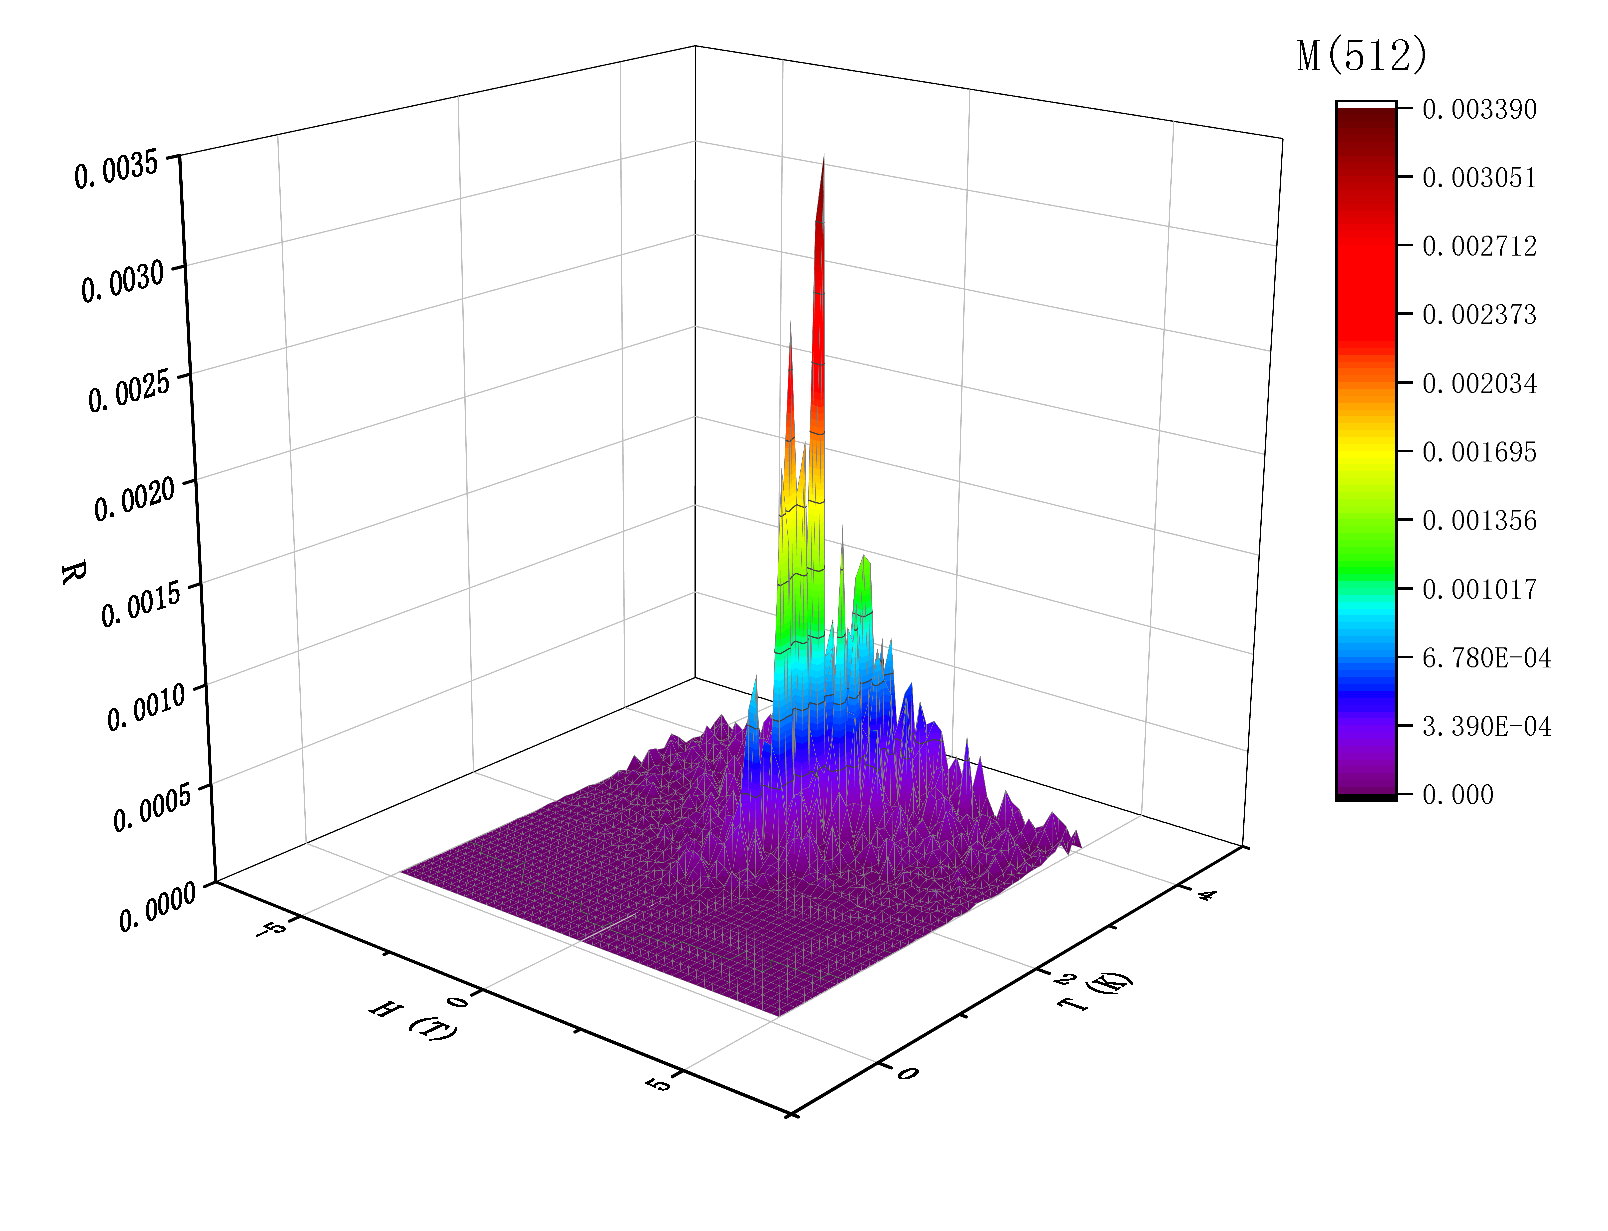
\includegraphics[width=5.5cm]{DeltaM-HT512.pdf}}\quad
                    \subfigure{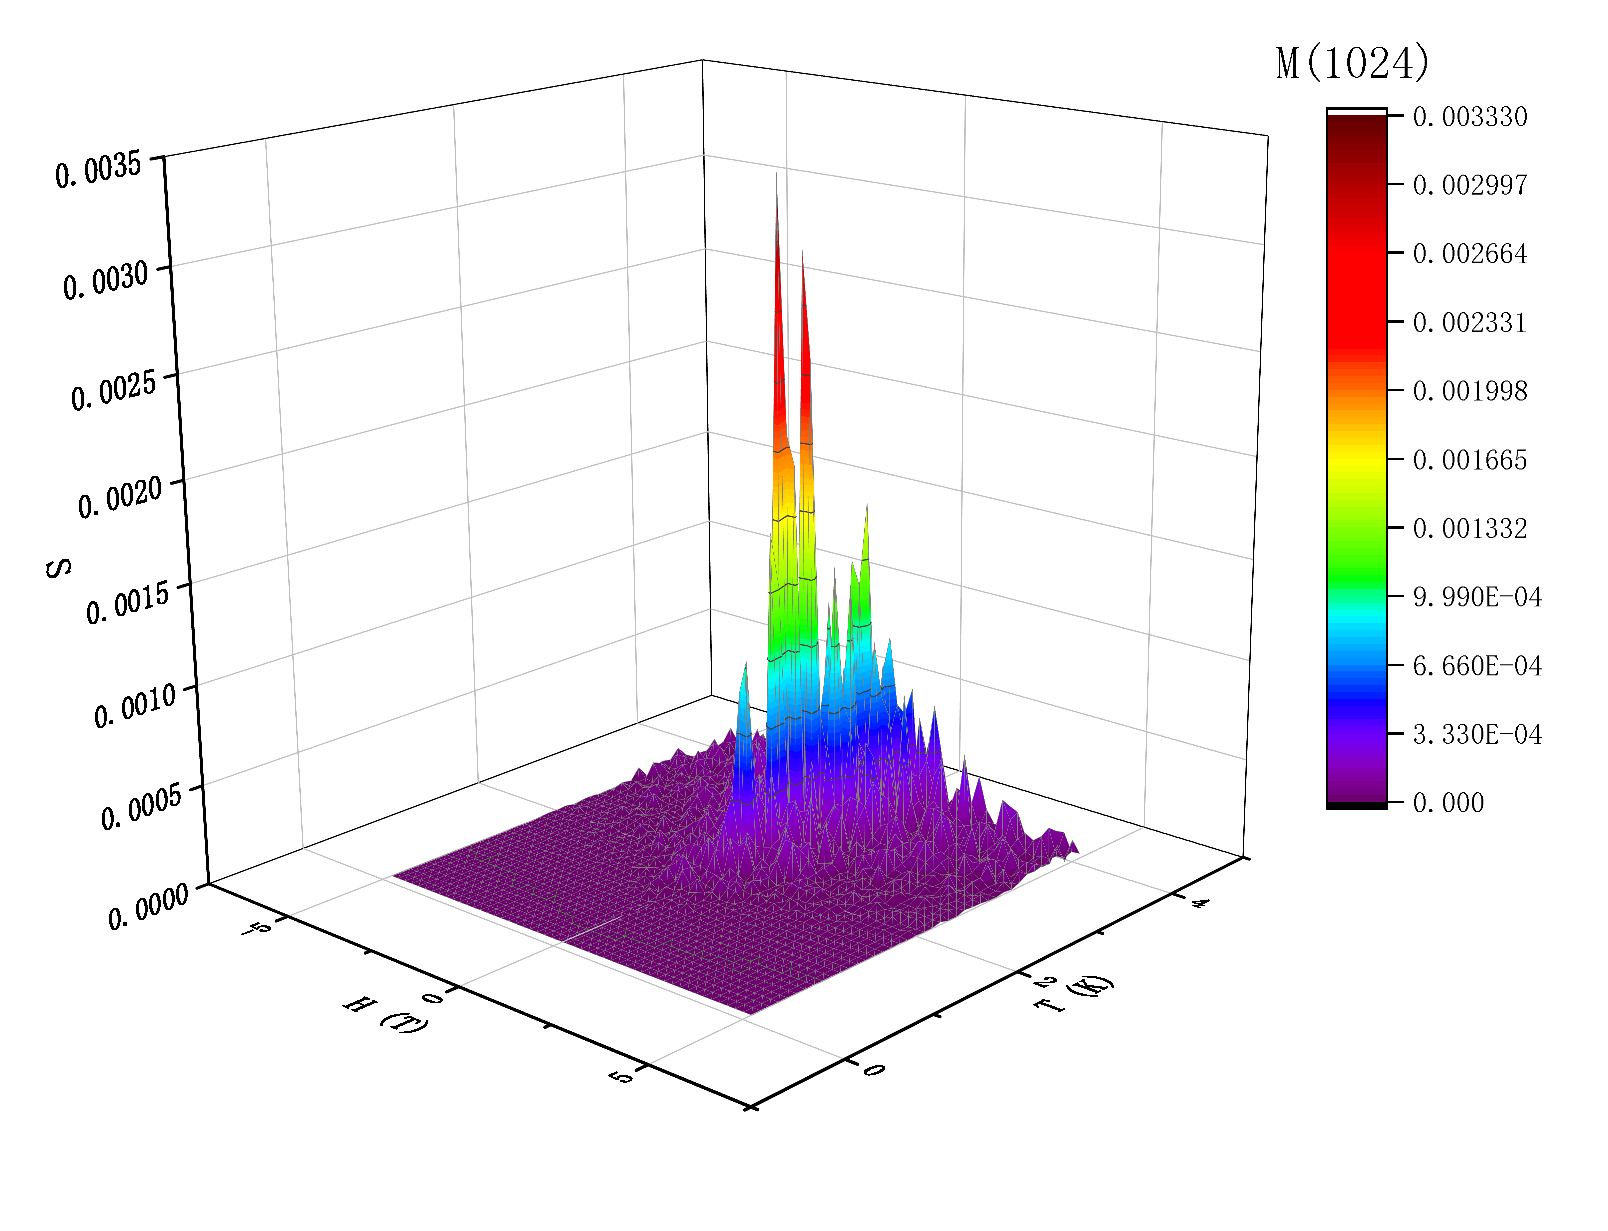
\includegraphics[width=5.5cm]{DeltaM-HT1024.pdf}}\quad
                    \subfigure{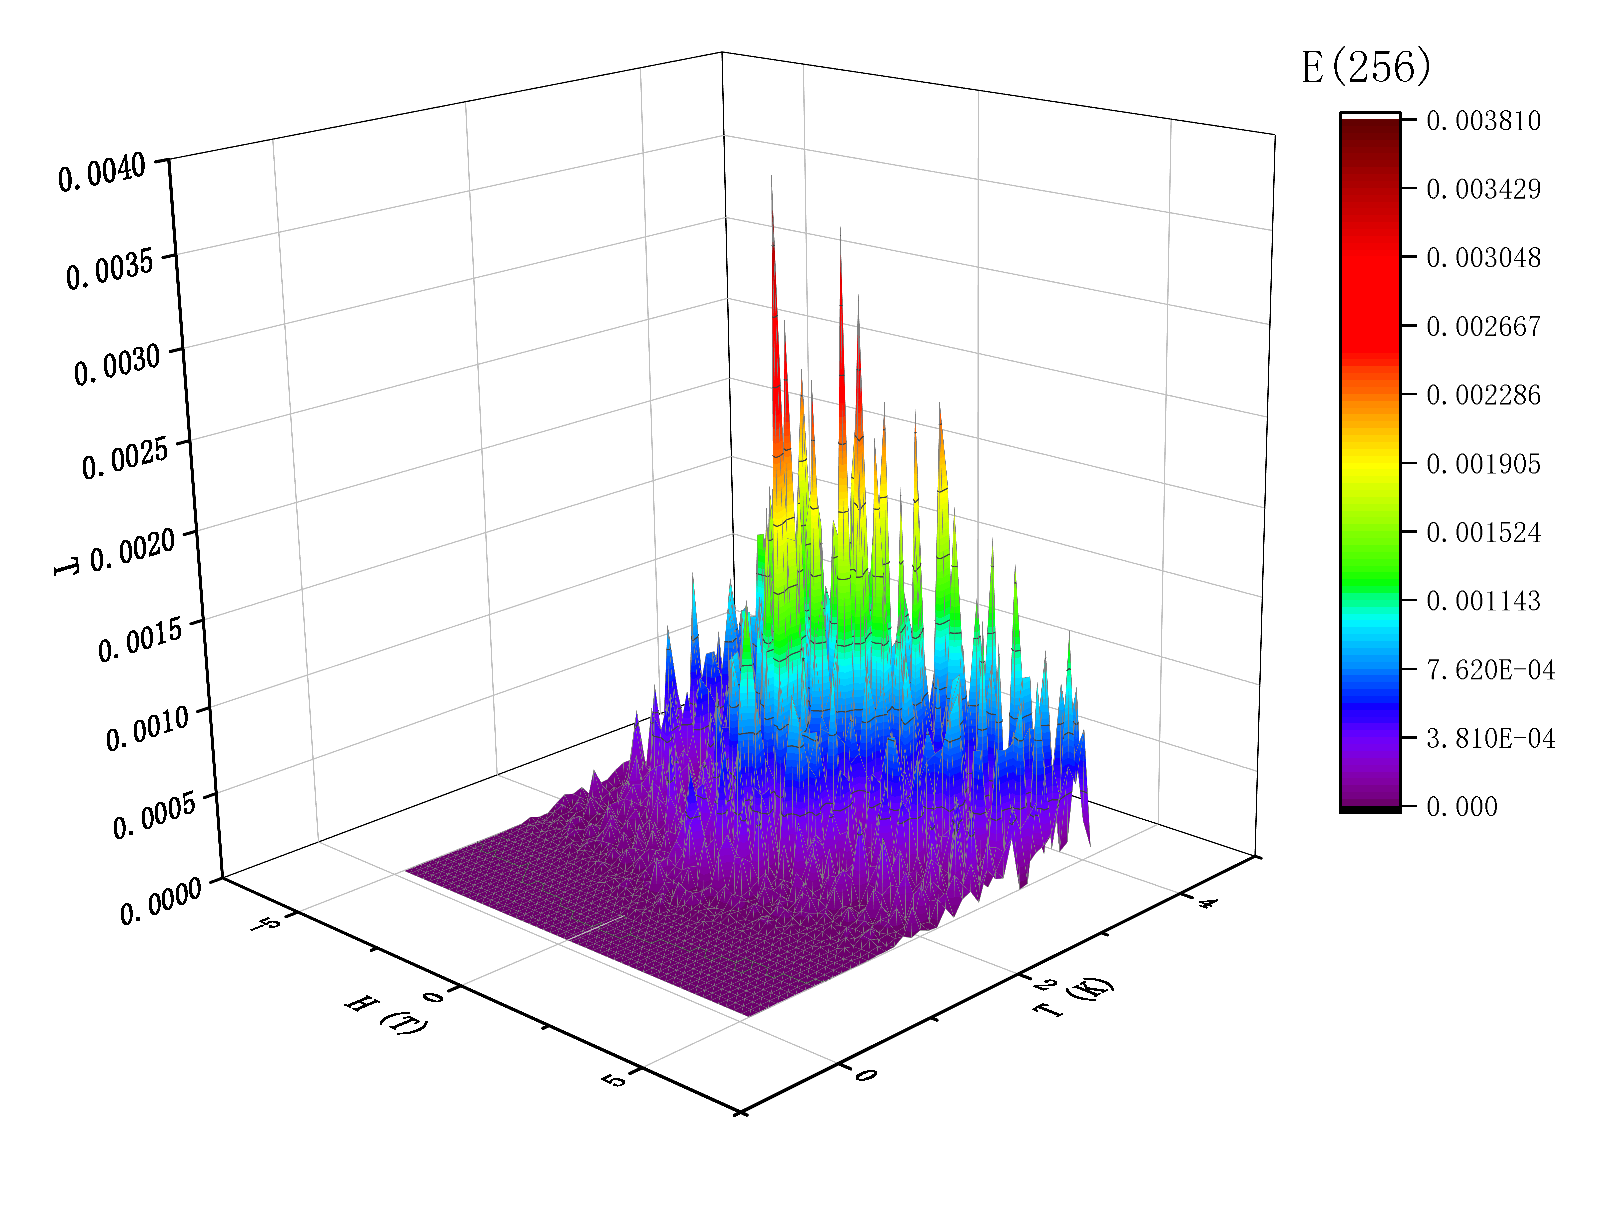
\includegraphics[width=5.5cm]{DeltaE-HT256.pdf}}\quad
                    \subfigure{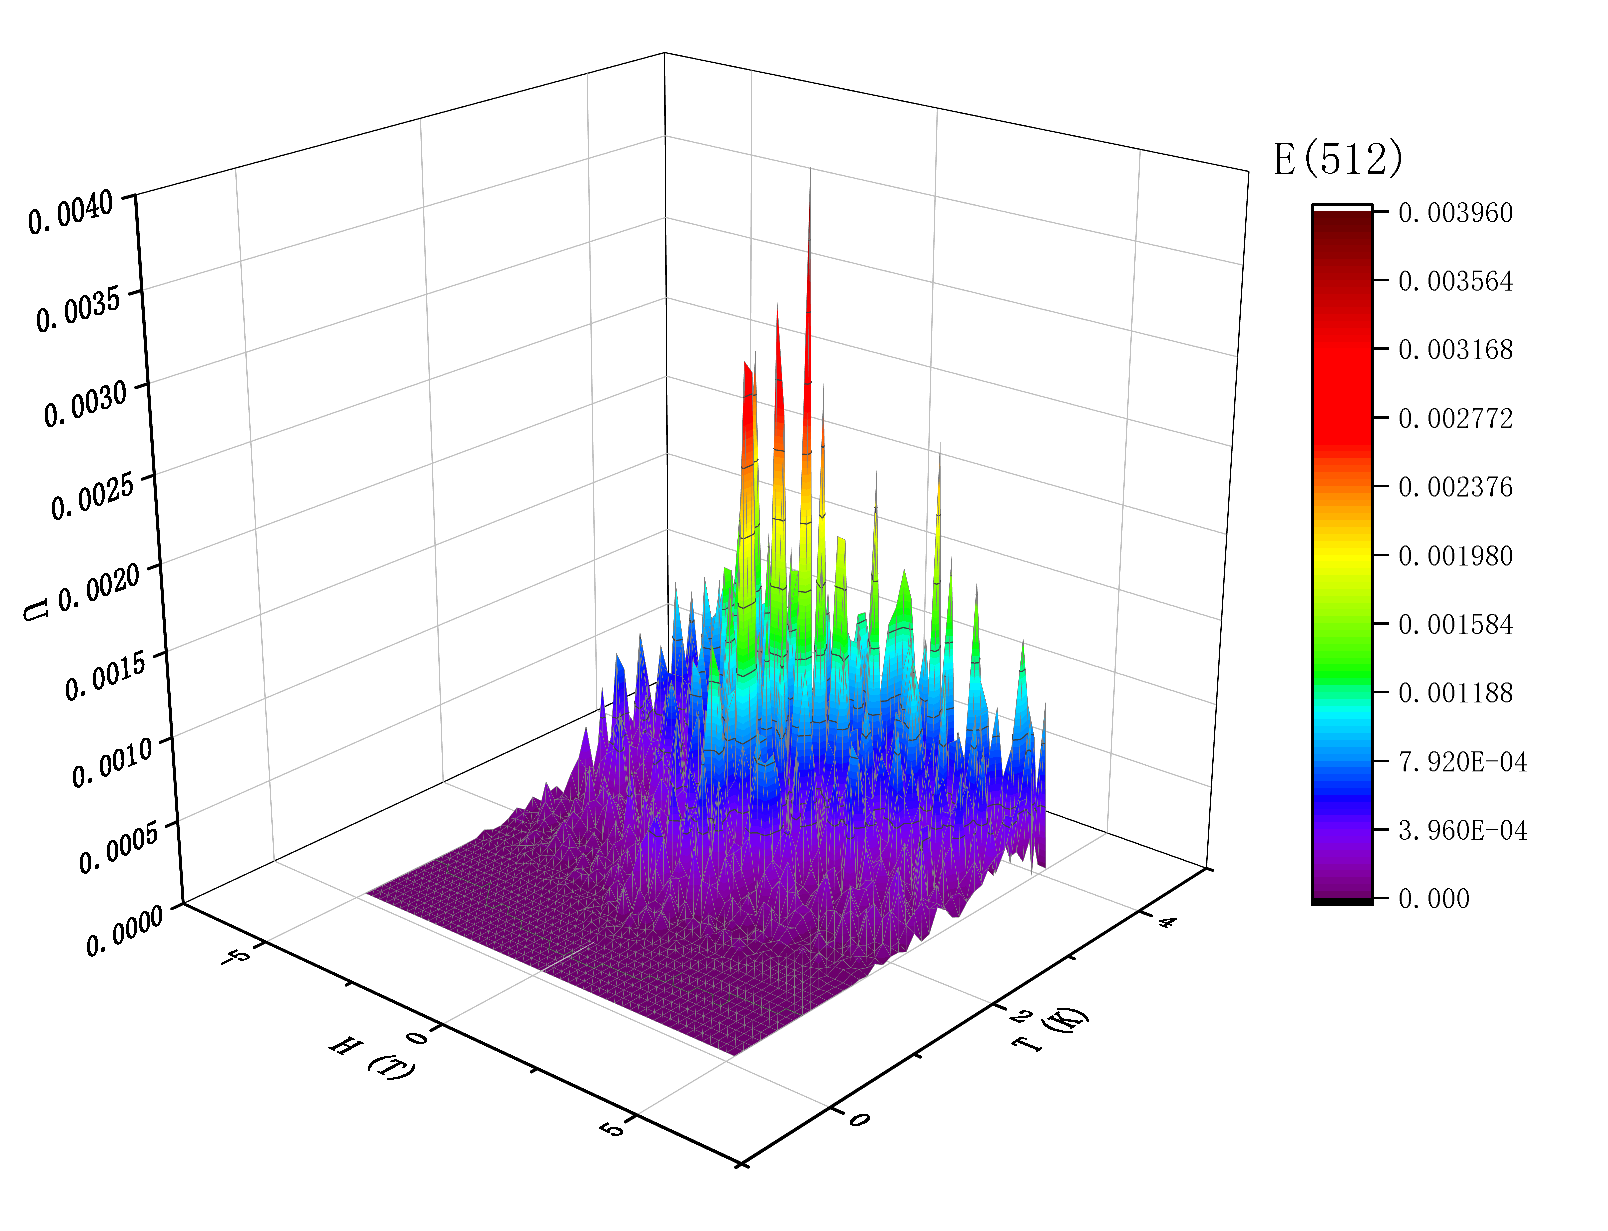
\includegraphics[width=5.5cm]{DeltaE-HT512.pdf}}\quad
                    \subfigure{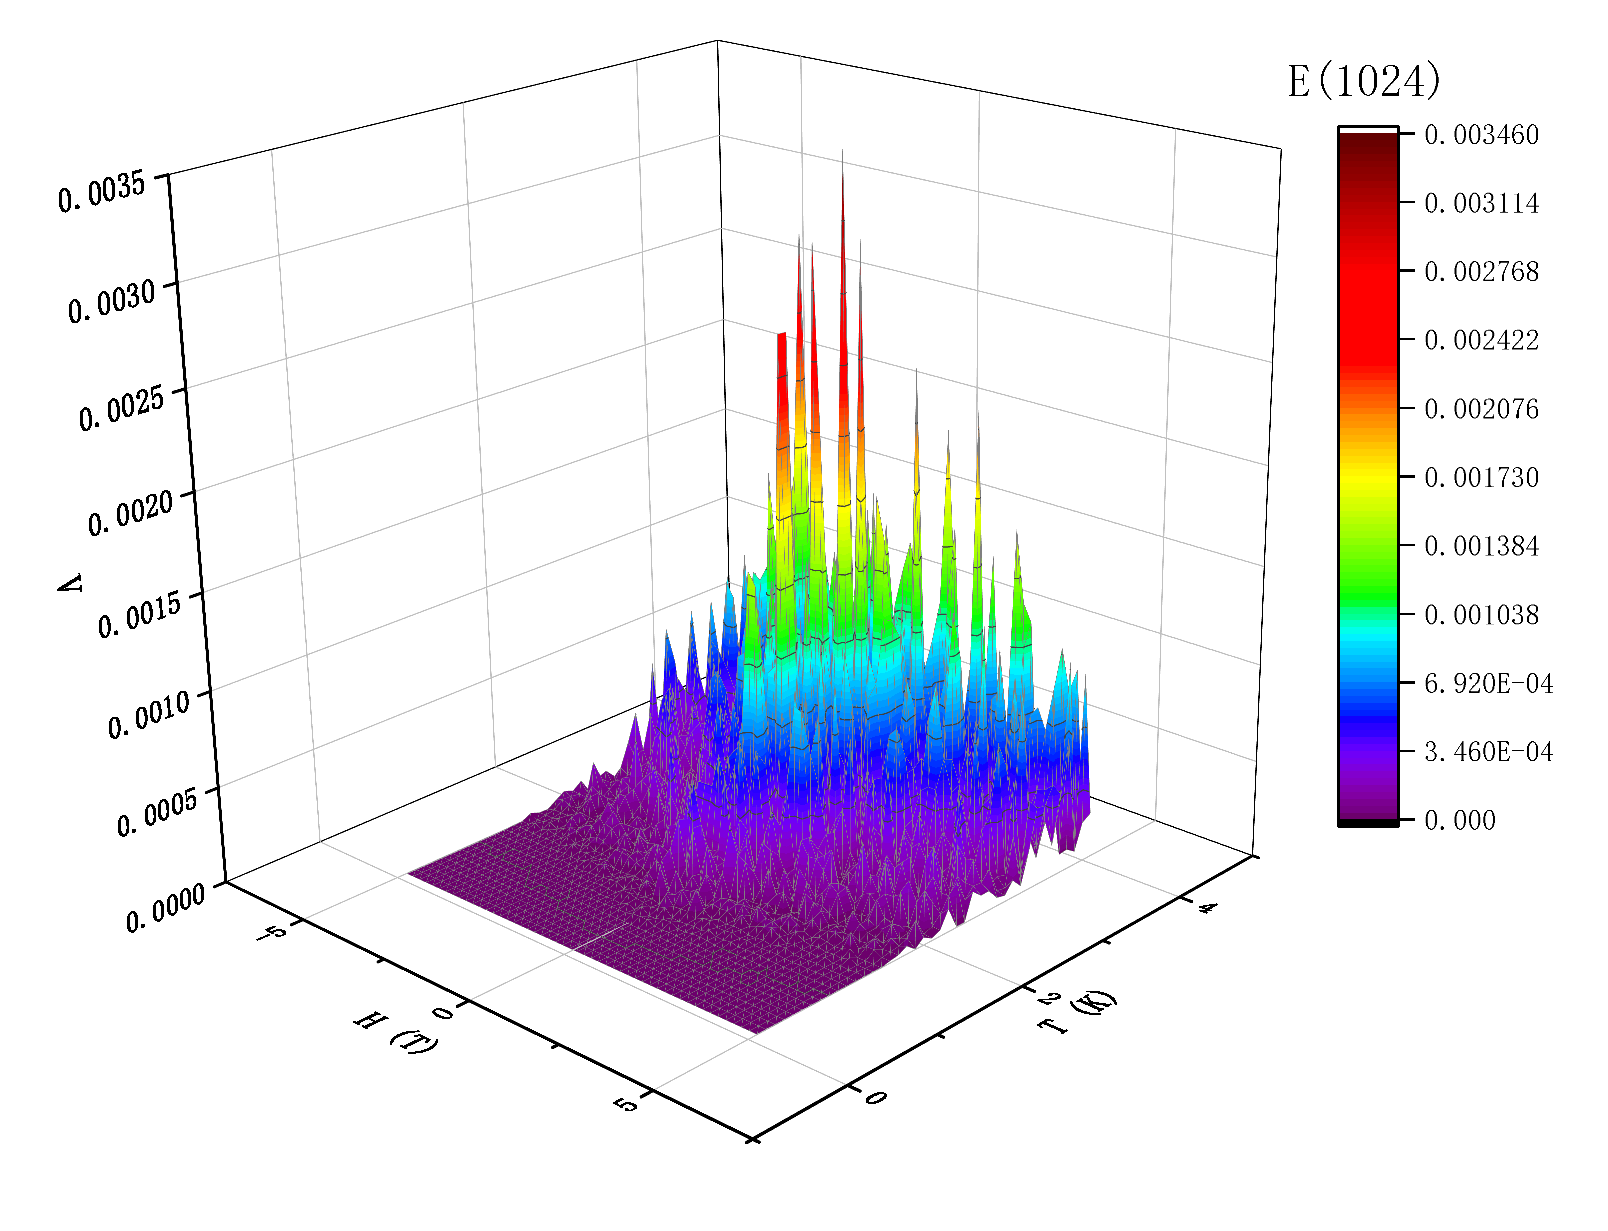
\includegraphics[width=5.5cm]{DeltaE-HT1024.pdf}}\quad
                \end{figure}
                可以看出误差基本上是在$10^{-3}$级, 而且这个误差还会随着系综平均的数量的增加而减小, 所以可以认为这几个尺寸网格计算得到的$M, E$是基本一致的. 这种性质要归功于
                周期性, 即使网格不够大也能被其周期性弥补而不至于受到边界条件的过大影响.
                \newpage
        \subsection{热容, 磁化率和熵}
            \subsubsection{热容}
                \indent $H=0.1$T的热容计算结果如下:
                \begin{center}
                    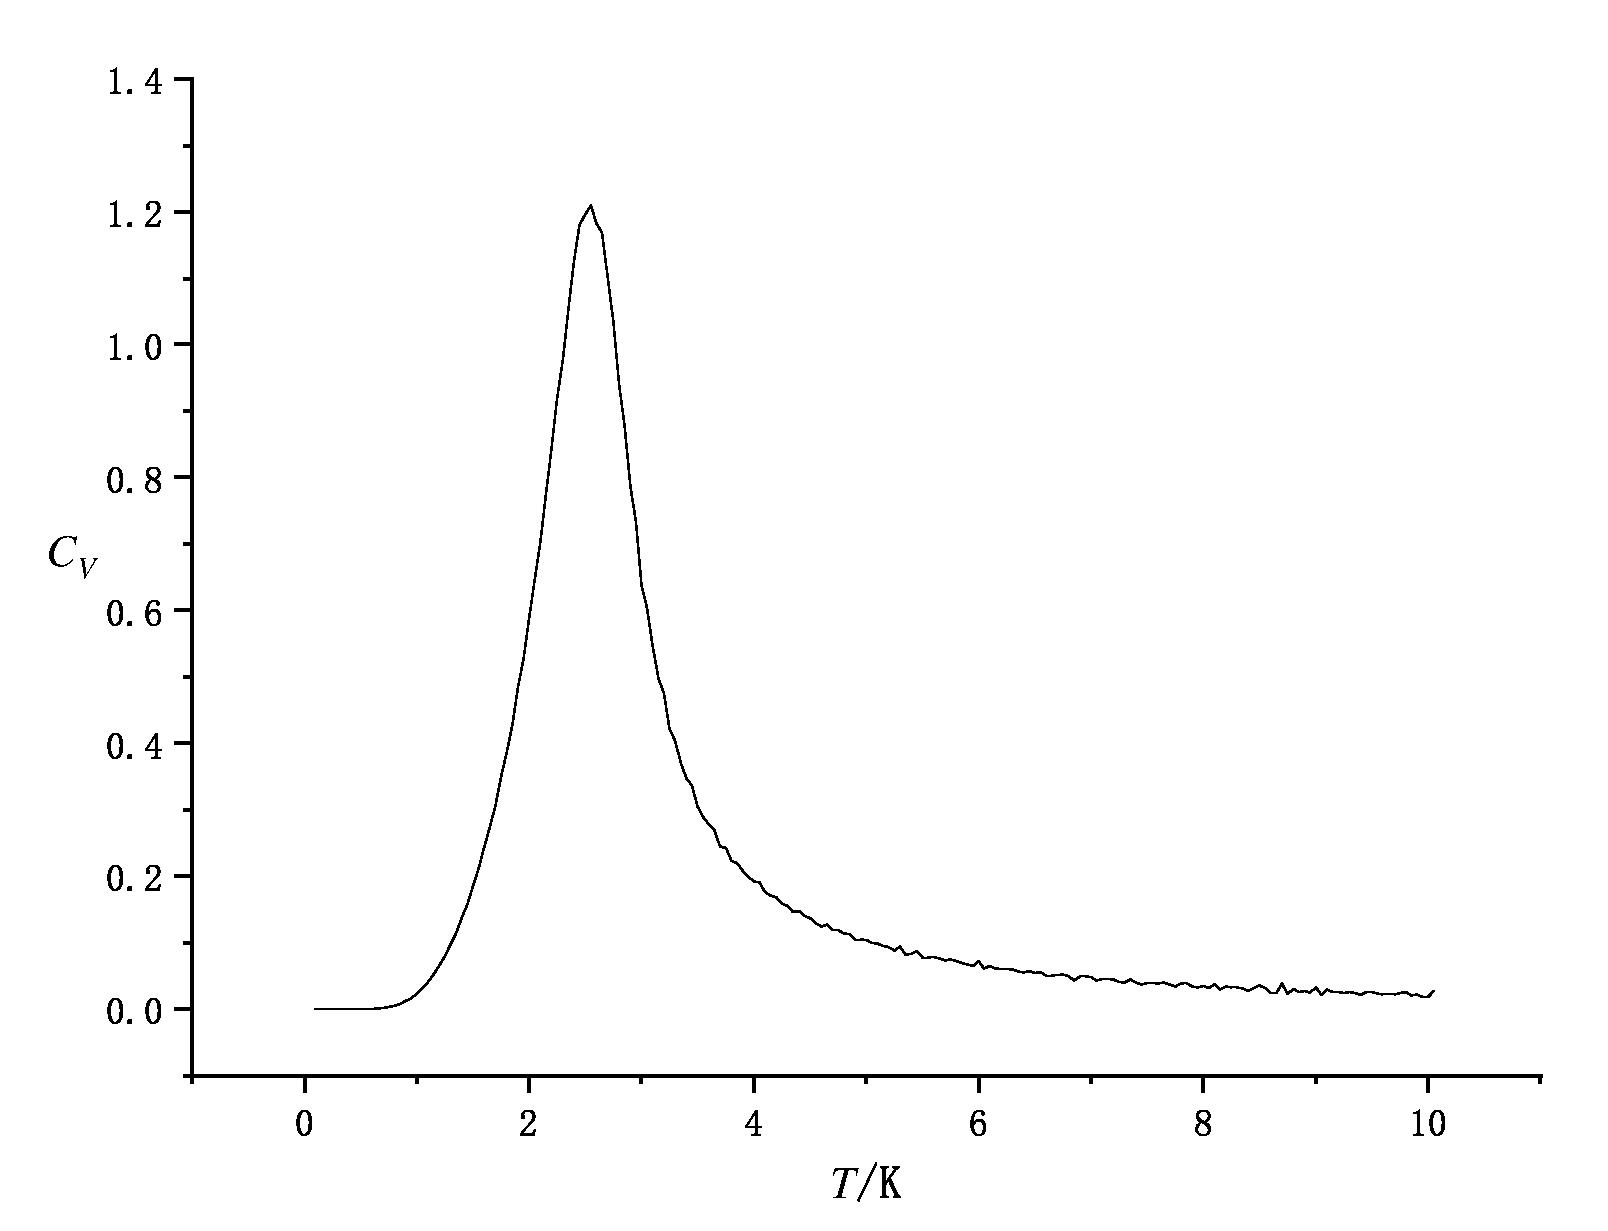
\includegraphics[width=13cm]{Cv-T.pdf}
                \end{center}
                可以看出在$T_c$附近有热容的极值.
            \subsubsection{磁化率}
                \indent $H=0.1$T得磁化率计算结果如下:
                \begin{center}
                    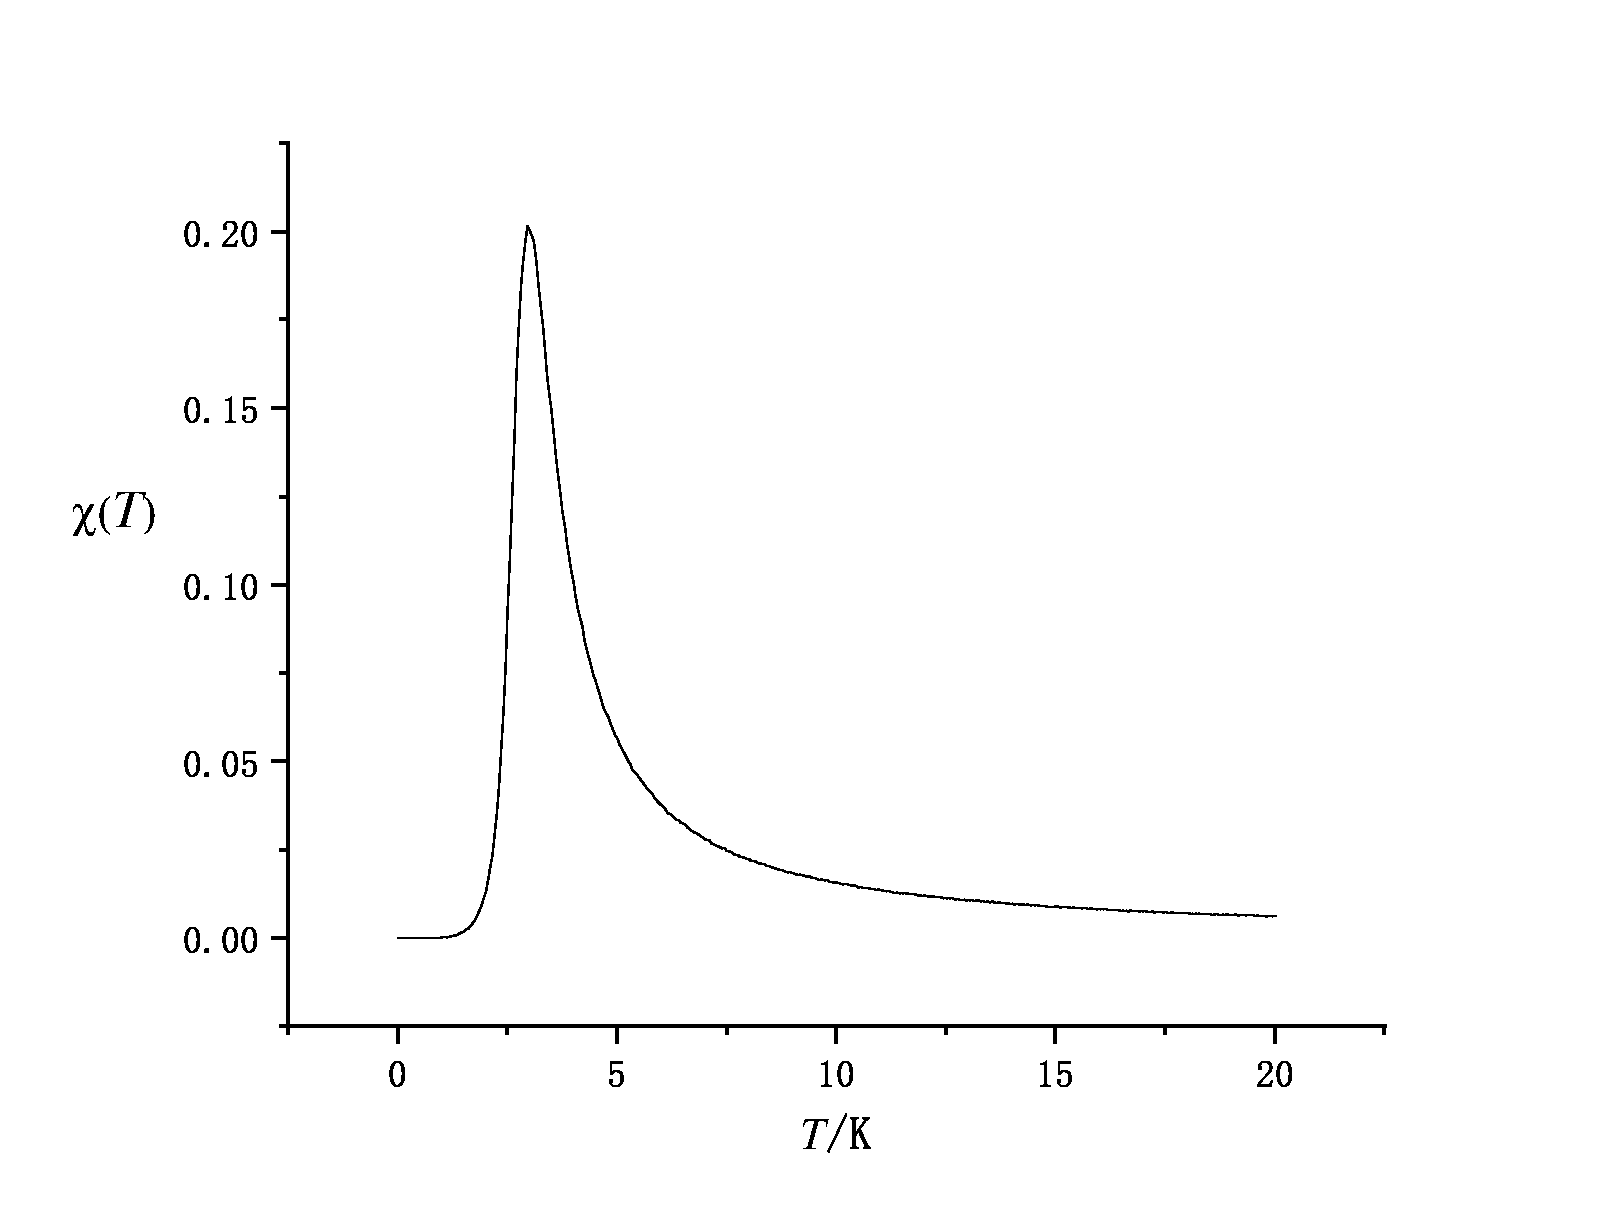
\includegraphics[width=13cm]{Chi-T.pdf}
                \end{center}
            \subsubsection{熵}
                \indent $H=0.1$T的熵计算结果如下:   
                \begin{center}
                    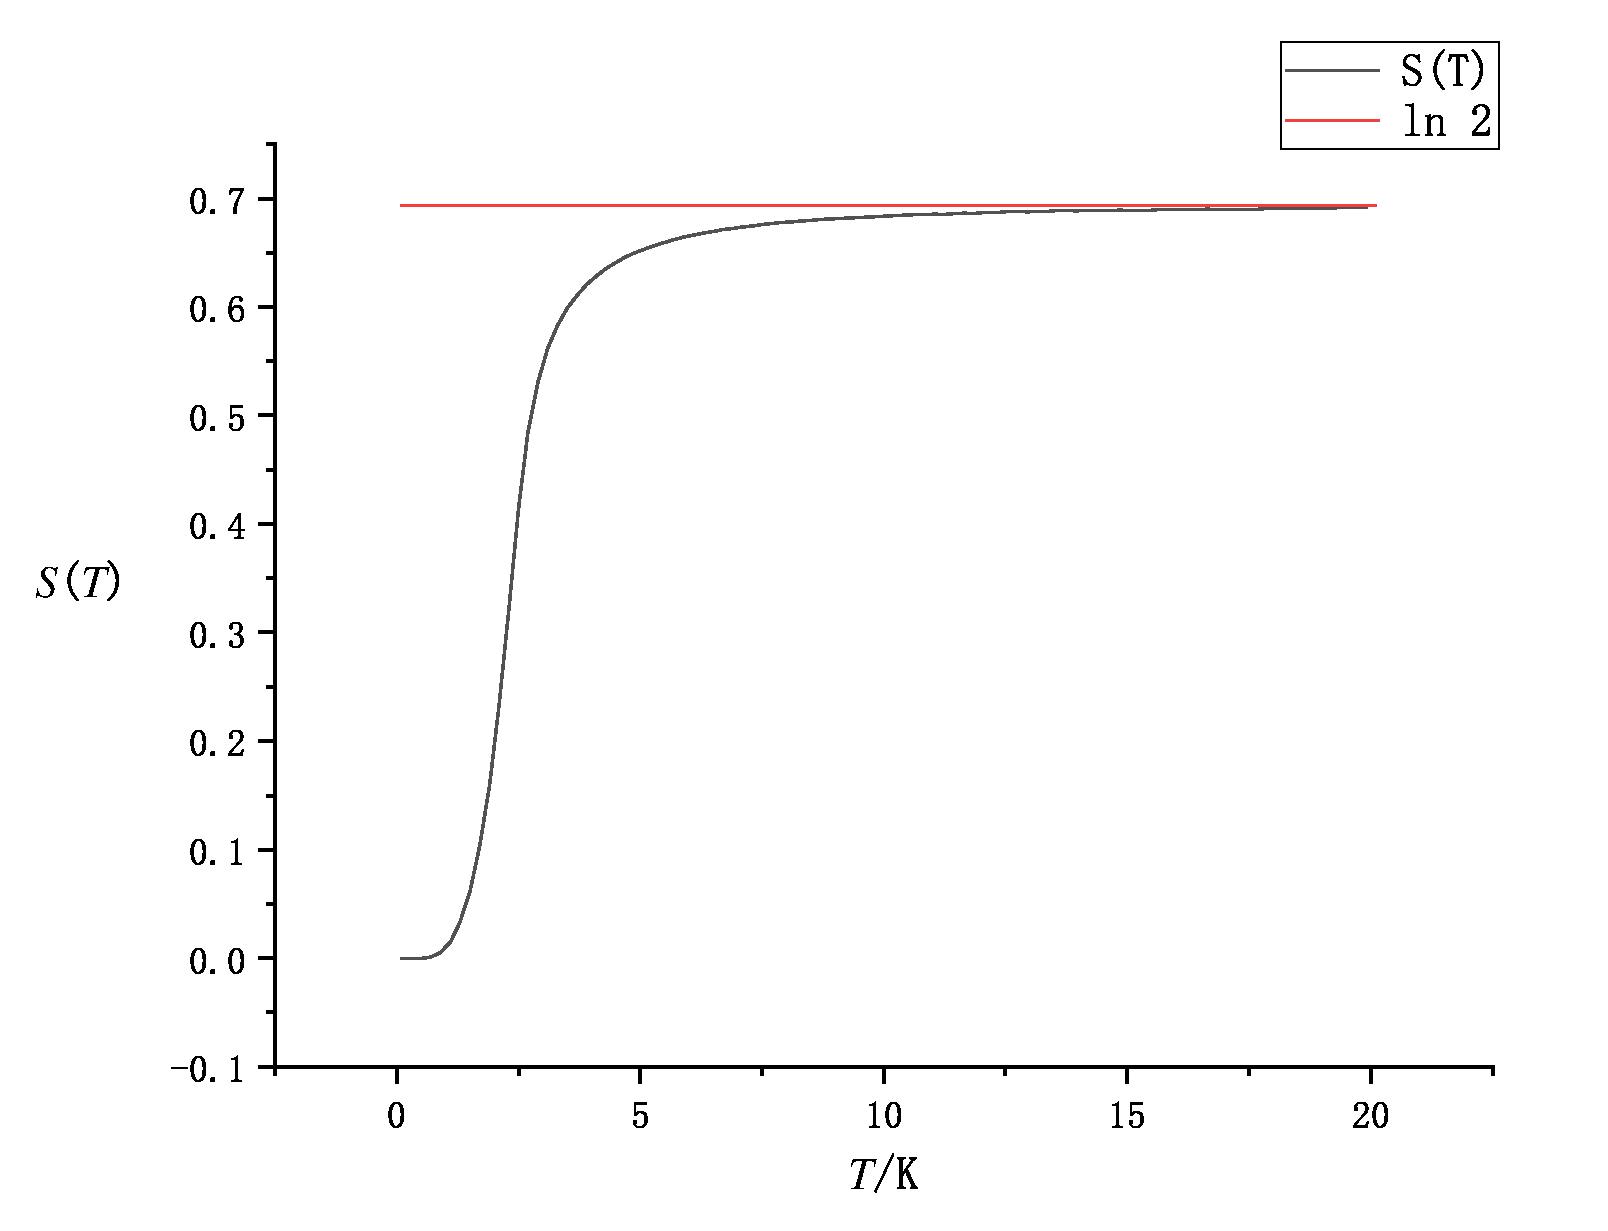
\includegraphics[width=13cm]{S-T.pdf}
                \end{center}
                这与系综理论得到的无穷温度下的熵为$Nk\ln 2$吻合得非常好.
                \newpage
        \subsection{零外场磁畴凝聚}
            \indent 在临界相变的温度下, 系统会出现类似小磁畴的现象, 即一团相邻的格点磁矩方向相同. 这种现象的出现与磁矩相互作用的局域性有关, 即近邻的磁矩 (铁磁性) 在低温时会趋向于
            同向而使能量最低, 但是这种凝聚会被高温激发翻转磁矩破坏.
            \subsubsection{网格尺寸对零外场磁畴凝聚的影响}
                \indent 猜想这种凝聚现象与网格尺寸有关. 为模拟一定时间下的平均, 这里取了10个紧邻系统 (通过连续翻转自旋得到) 的平均. 以下是4个尺寸下在温度为2.3K的凝聚现象:
                \begin{center}
                    \includegraphics[width=17cm]{4_Size_Grids.pdf}
                \end{center}
                从图中可以看出磁畴尺寸基本上是随着网格大小的增大变大的, 这是由于网格的周期边界条件会影响到了大尺寸磁畴的产生, 因为周期频率很低的大磁畴是无法存在于小网格中的.
                \newpage
            \subsubsection{温度对零外场磁畴凝聚的影响}
                \indent 显然这种结构的出现于温度是息息相关的, 因为在温度较低的时候, 系统的一大块磁畴的能量足够低足够稳定, 而随着温度的升高, 这种大块的结构会因为其中的磁矩受到热激发翻转
                而被破坏, 所以大块的磁畴会逐渐分解成小块的. 以下模拟验证了这种结果:
                \begin{center}
                    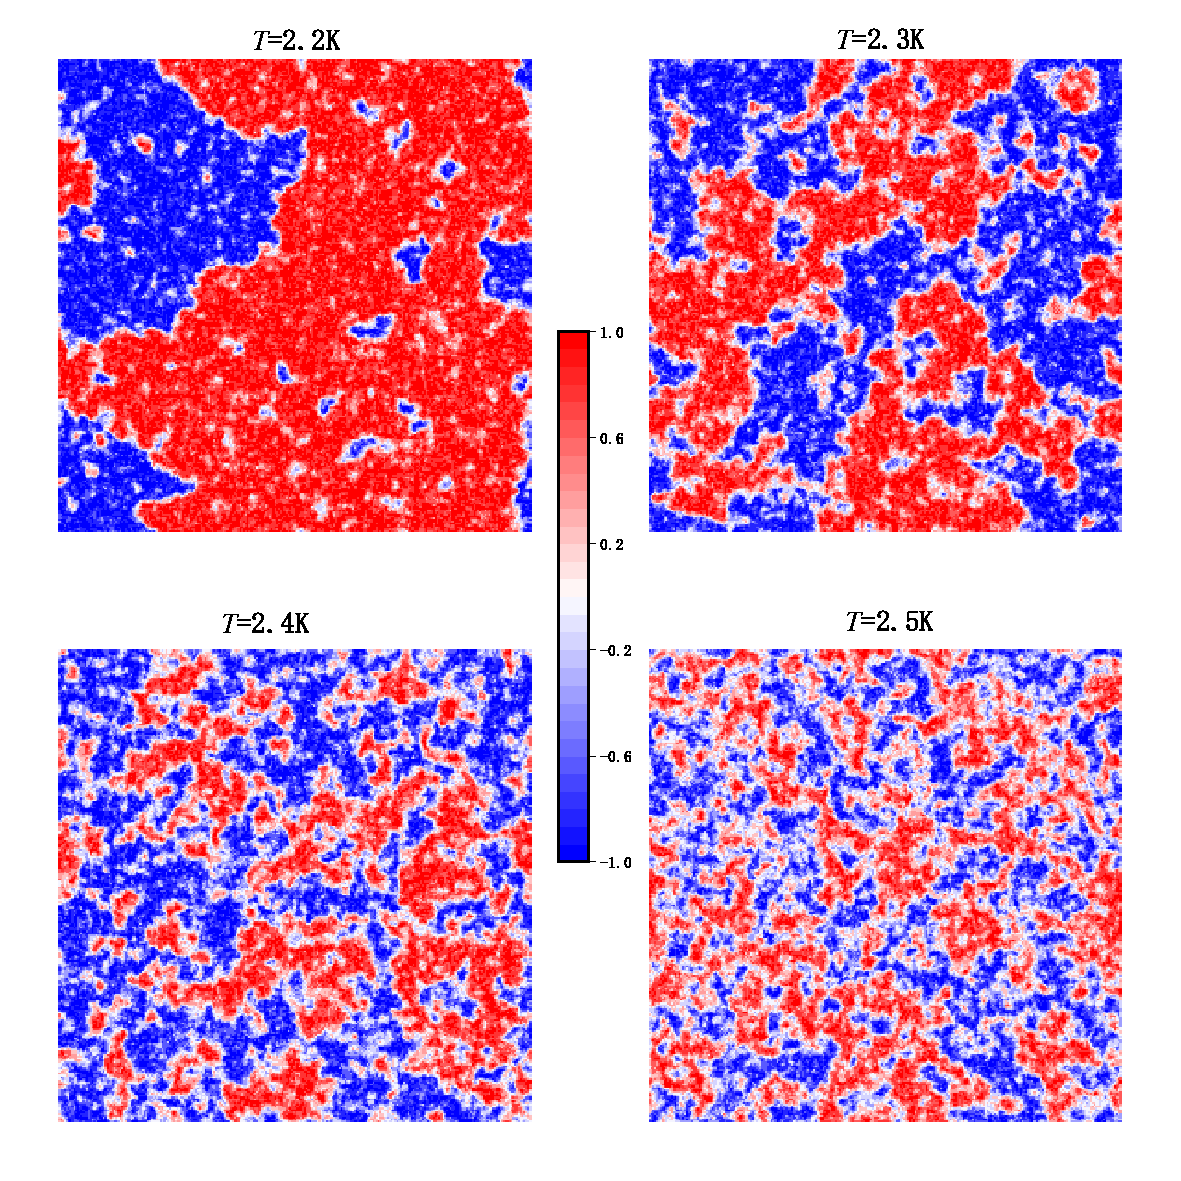
\includegraphics[width=17cm]{4_T_Grids.pdf}
                \end{center}
                \newpage
            \subsubsection{平均时间对零外场磁畴凝聚的影响}
                \indent 显然这种磁畴是会随着自旋的不断翻转而逐渐产生, 消失和移动. 所以随着平均时间的增加, 自旋翻转会使得不同区域磁矩的时间平均值趋于一致.
                从模拟结果可以看出这种移动其实是十分缓慢的, 在很长一段时间内磁矩的时间平均仍然会出现局域性. 当然这种局域的尺寸会比磁畴的尺寸大很多,
                因为磁畴的移动会抹平高频的边界.
                \begin{center}
                    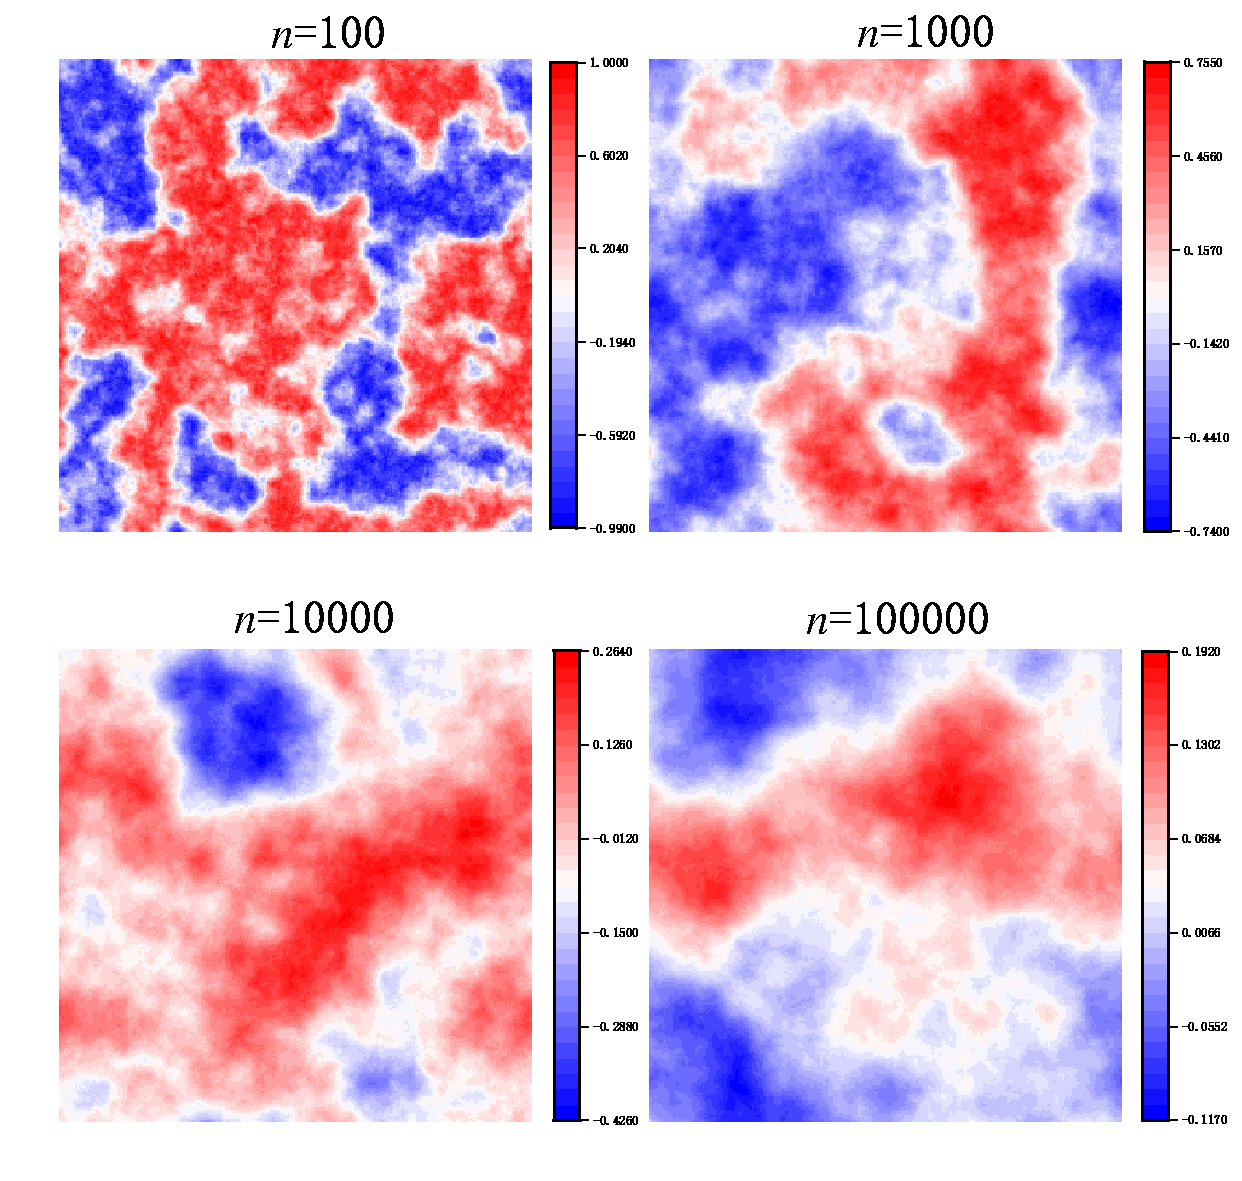
\includegraphics[width=17cm]{4_Num_Grids.pdf}
                \end{center}
                \newpage
        \subsection{磁滞曲线的模拟}
            \indent 由于Ising模型可以较好的模拟实际铁磁体的各种性质, 所以这里选择一种铁磁体的典型行为--磁滞曲线进行模拟.
            这里模拟的方式是:\\
            \indent 首先由随机状态达到极值磁场下的平衡态 ($T<T_c$), 即磁矩是同向的, 再逐渐步进减小磁场, 每减小一次就重新达到一次平衡, 然后记录多个个系综的平均值作为总磁矩,
            直至磁场达到反向极值, 再反过来重复以上过程. 以下是在不同温度下的模拟结果:
            \begin{center}
                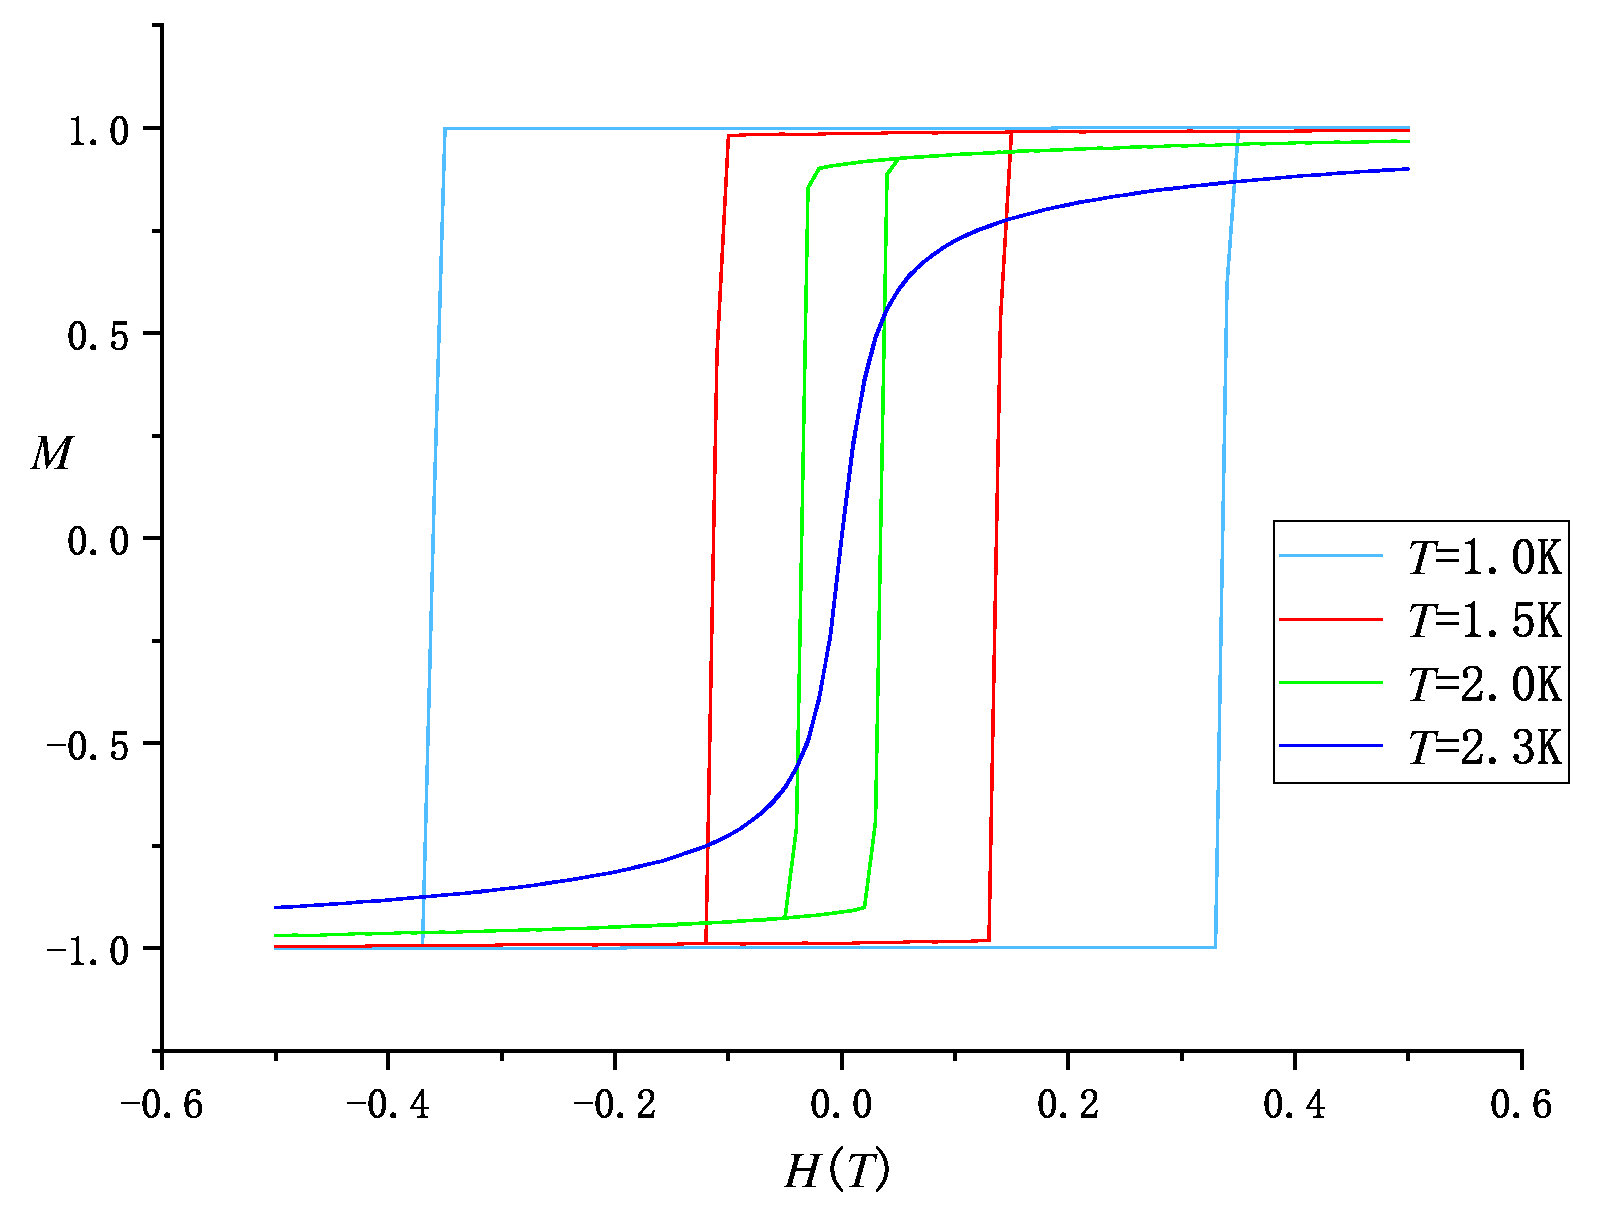
\includegraphics[width=17cm]{HysteresisCurve.pdf}
            \end{center}
            可以看出与实际的磁滞曲线十分相似, 而且在高温时从铁磁介质转变为顺磁介质这种现象也十分明显.
    \section{结论}
        \indent 经过以上计算结果表明, 虽然伊辛模型是一个十分简单的解释自旋相互作用系统的模型, 但是其在不同温度下的统计规律却能反映丰富的物理内涵, 值得进行数值模拟, 以便验证系综理论的正确性.
        而这仅仅是一个简单的二维系统, 若推广到三维乃至更高维, 相信还会出现更多精细现象. 而模拟的方法梅特波斯利算法本身就是一个适用性很广的方法, 在各个领域都有应用.
\end{document}